% !TEX TS-program = pdflatex
% !TEX encoding = UTF-8 Unicode

% This is a simple template for a LaTeX document using the "article" class.
% See "book", "report", "letter" for other types of document.

\documentclass[11pt]{article} % use larger type; default would be 10pt.
\setcounter{secnumdepth}{2}


\usepackage[utf8]{inputenc} % set input encoding (not needed with XeLaTeX)
\usepackage{float} % to place float images correctly
\usepackage{color} % to color text

%%% Examples of Article customizations
% These packages are optional, depending whether you want the features they provide.
% See the LaTeX Companion or other references for full information.

%%% PAGE DIMENSIONS
\usepackage{geometry} % to change the page dimensions
\geometry{a4paper} % or letterpaper (US) or a5paper or....
% \geometry{margin=2in} % for example, change the margins to 2 inches all round
% \geometry{landscape} % set up the page for landscape
%   read geometry.pdf for detailed page layout information

\usepackage{graphicx} % support the \includegraphics command and options

% \usepackage[parfill]{parskip} % Activate to begin paragraphs with an empty line rather than an indent

%%% PACKAGES
\usepackage{booktabs} % for much better looking tables
\usepackage{array} % for better arrays (eg matrices) in maths
\usepackage{paralist} % very flexible & customisable lists (eg. enumerate/itemize, etc.)
\usepackage{verbatim} % adds environment for commenting out blocks of text & for better verbatim
\usepackage{subfig} % make it possible to include more than one captioned figure/table in a single float
% These packages are all incorporated in the memoir class to one degree or another...

%%% HEADERS & FOOTERS
\usepackage{fancyhdr} % This should be set AFTER setting up the page geometry
\pagestyle{fancy} % options: empty , plain , fancy
\renewcommand{\headrulewidth}{0pt} % customise the layout...
\lhead{}\chead{}\rhead{}
\lfoot{}\cfoot{\thepage}\rfoot{}

%%% SECTION TITLE APPEARANCE
\usepackage{sectsty}
\allsectionsfont{\sffamily\mdseries\upshape} % (See the fntguide.pdf for font help)
% (This matches ConTeXt defaults)

%%% ToC (table of contents) APPEARANCE
\usepackage[nottoc,notlof,notlot]{tocbibind} % Put the bibliography in the ToC
\usepackage[titles,subfigure]{tocloft} % Alter the style of the Table of Contents
\renewcommand{\cftsecfont}{\rmfamily\mdseries\upshape}
\renewcommand{\cftsecpagefont}{\rmfamily\mdseries\upshape} % No bold!
\newcommand{\pe}{PowerEnJoy }
\newcommand{\pecomma}{PowerEnJoy, }

%%% END Article customizations

%%% The "real" document content comes below...




\title{Requirements Analysis and Specifications Document (RASD)}
\author{Simone Mosciatti \& Sara Zanzottera}

\begin{document}
\maketitle
\newpage
\tableofcontents
\newpage


\section{Introduction}

In this section we are providing an overview of the \pe Project, we are highlighting what the product does, what functions it provides, what constrains it has and what assumption we made during the design process.

  \subsection{Purpose}
  
The purpose of this document is to analyze the requirements for the project and provide detailed specifications for \pecomma a digital management system for a car sharing service that features only electric cars.
  
  \subsection{Scope}
  
\pe is a car sharing platform focused exclusively on eletric cars. It aims to improve the mobility inside the city in a eco-friendly way. To achieve its goal, it will incetivize people to be environment cautions drivers.

\subsection{Definitions, acronyms, abbreviations}
  \begin{description}
  	\item[GPS]: Global Positioning System is a global navigation satellite system (GNSS) that provides location and time information in all weather conditions, anywhere on or near the Earth where there is an unobstructed line of sight to four or more GPS satellites.
  	\item[Running Time] The time that an user is using the \pe service.
  	\item[Frontend]
  	\item[Backend]
  \end{description}
  
\subsection{Overview}

\section{Overall Description}

\pe is a digital management system for car sharing that exclusively employs electirc cars to provide its service. The system provides all the functionalities normally provided by a car sharing service, like registering to the service, find the location of nearby available cars, reserve cars up to a short amount of time (namely one hour), unlock the chosen car once found, ride it and then park it in a safe area, when it will be automatically locked and the fee paid.

In addition, the system gives bonuses and penalities in term of discounts or extra fees depending on the behavior of the user, in order to incentivize a virtuous behavior. Some examples are:

\begin{itemize}
	\item a discount of 10\% for users who brings other passangers with him during the ride
	\item a discount of 20\% if the car is left with at least 50\% of the battery still full, or a 30\% if the car is left near a charging station and plugged.
	\item if the car is left more than 3km from the nearest charging station or with less than 20\% of charge left, the user is charged 30\% more
\end{itemize}

\pe is divided in two main part: a frontend, used by the customers, and a backend that provides the service. In addition there is a reserved fronted, used exclusively by the staff members to better organize their job.


\subsection{Product Perspective}
  
  \pe provide users the ability to rent cars for a limited amount of time in a bounded area, for example a city. 
  The frontend part, the app, provides the user the ability to look for available cars, reserve cars for up of one hour and unlock the cars once they are near the reserved vehicle; it is used also to lock the vehicle once the run is over and to pay the fee.

The staff's reserved frontend tells them which cars need to be plugged or recharged in-place, which cars need to be brought to a safe parking area, or if some users need help for some technical issue with their car. It also provides them with the ability of registering fines sent to the company by local police officers, as for the system to assign them to the correct user to pay.

  The backend part takes care of providing all the required data to both frontends. It also tracks the position and the statuses of every single car, the duration of each ride and charges users accordingly.
  
\subsection{Product Functions}
  
  \pe is provided to the user via a mobile application. A registered user can log in into its account, while a new user is prompted to register and then to log in.
  
  After the user logged in they will be able to see the position of each car in the city or in a more strictly bounded area, for example, within ten minutes by foot. Once the user has decided which car he wants to use, they will be able to book the car for one hour. After the car is been booked, the user can unlock the car only when in proximity of the car itself.
  
  The system starts charging the user when the engine starts running, and will stop once the car is been parked, the user exit and locks it. Several forms of discount or overfees will be applied depending on the behaviour of the user when riding and parking the car.


\subsection{Parallel Operation}
  The system is capable to operate and serve users concurrently, however an, HA, single point of coordination is required in order to avoid conflicts on the booking system.
 
\subsection{Constraints}
  
	\subsubsection{Constraints on the user}
Users who wish to use \pe are required to fulfill some specific requirements:
\begin{enumerate}
	\item The user must be registered to the service.
	\item The user must have a valid driving license.
\end{enumerate}

	\subsubsection{Platform Contraints}
Also, the system has some platform constraints coming from the device that is running the app:
\begin{enumerate}
	\item The app should be small enough to fit the memory of ideally all smartphones.
	\item The app should be thin enough to fit the computational capabilities of ideally all smartphones.
	\item The app should send and receive only small quantity of data through the smartphone's internet connection, in order to be sustainable.
	\item The app should be able to get information from the smartphones' GPS.
  \end{enumerate}

	\subsubsection{Privacy regulations}
The system should complain to the most recent privacy regulations in managing the data that the user are generating, thus ensuring:
\begin{enumerate}
	\item The user must be aware that its data is being recorded by the system, including its GPS position.
	\item The user must be able to see which data the system collected about him and, in case, to delete it (even if this may require the user to unsubscribe from the service
).
	\item No third parties should be able to gain access on users' data.
	\item Users' data must be protected from third-parties attacks.
	\item Users' data should not be possible to obtain by reverse-engineering the behavior of the system.
\end{enumerate}

\subsection{Actors and stakeholders}

\subsubsection{Actors}
The actors involved in our system are mainly \textbf{final users}, that is, people who are renting cars. Indeed the system needs support from a \textbf{technical team} that takes care of the digital infrastructure, and a \textbf{staff} that takes care of the cars in some special situations:
\begin{itemize} 
	\item Cars left far from the power grid with an empty battery, that needs to be charged in-place
	\item Cars left far from a safe parking area, that needs to be brought back to one of them
	\item Cars not plugged to the power grid, that needs to be plugged
	\item Cars which has been reported by the user or by the onboard system itself having some technical issues
	\item Fines received by the company that needs to be assigned to the correct user
\end{itemize}

\subsubsection{Stakeholders}
The main stakeholder for our system are \textbf{users} themselves, who requires a easy-to-use service of electric cars sharing. Other stakeholders are the \textbf{city governement}, who supports our service as a way to improve sustainable mobility inside the city and takes care of the road infrastructures, and the \textbf{energy companies}, which provide power for the cars.

\subsection{Text Assumptions}

\subsubsection{Assumptions on the final user}
\begin{enumerate}
	\item The final user has reached the legal age and has a driving licence
	\item The final user has a smartphone with the \pe app installed
	\item The final user has a smartphone with a GPS
	\item The final user has a smartphone with internet connectivity
\end{enumerate}
  
\subsubsection{Assumptions on the car system}
\begin{enumerate}
	\item  Each car is provide with internet connectivity and capable to send and receive data to the main server
	\item  Each car is provided of a GPS of reasonable accurancy.
	\item  Each car can capture all these events correctly:
		\begin{itemize}
			\item the ignition of the engine
			\item the status of the engine
			\item the users getting into the car
			\item the users exiting the car 
			\item the number of passengers.
			\item the user plugging the battery to the power grid.
			\item the locked status of a car
		\end{itemize}
	\item Each car is able to monitor the residual charge of its battery.
	\item Each car is provided with a device that can scan and read a driving licence.
	\item The system is able to prevent the ignition of each car's engine remotely.
	\item The system is able to switch off every car's engine remotely.
	\item The system is able to unlock each car remotely.
	\item The system is able to lock each car remotely.
	\item An empty car gets locked automatically after a short time (namely 5 minutes)
\end{enumerate}

\subsubsection{Statuses assumptions}
The cars are assumed to have some internal, discrete statuses describing their conditions. These are:
\begin{itemize}
	\item{Availability Status}: describe if the car is interacting with some users of if it is available for rent. Possible values:
		\begin{itemize}
		\item Available
		\item Booked
		\item Unlocked
		\item Running
		\item Parked
		\item Not Available
		\end{itemize}
	\item{Charging Status}: describe if the car is connected to the power grid or not. Boolean values (True or False)
	\item{Locked Status}: describe if the car can be accessed by a person or not. Boolean values (True or False)
	\item{Exception Status}: describe if the car has some issues. Possible values are:
		\begin{itemize}
		\item No Issue
		\item Out Of Power
		\item Unsafely Parked
		\item Out of City Boudaries
		\item Technical issue
		\item Mechanical issue
		\item Other issue
		\end{itemize}
\end{itemize}
Here we list some text assumptions about these parameters.
\begin{itemize}
	\item The Availability status can change to Booked only if it was Available.
	\item The Availability status can change to Unlocked only if it was Available.
	\item The Availability status can change to Running only if it was Unlocked or Not Available. The latter case is possible only if the Exception status was Out of City Boundaries.
	\item The Availability status can change to Parked only if it was Running.
	\item  The Availability status can change to Available only if it was Parked or Not Available.
	\item The Availability status of a car with less than 20\% of residual charge is Not Available regardless of the status it was supposed to have, and its Exception status is set to Out Of Power.
	\item The Availability status of a car parked outside a safe area is Not Available and its Exception status is set to Unsafely Parked.
	\item The Charging status of a car can be True only if the car is plugged to the power grid.
	\item If Charging status is True, the charge must increase in time. Otherwise, the Availability status must be set to Not Available and the Exception status must be set to Mechanical Issue. 
	\item The Charging status of a car cannot be set to True if the Availability status of the car is Running. Otherwise, the Availability status must be set to Not Available and the Exception status must be set to Mechanical Issue. 
	\item if the Availability status of the car is different from Not Available, the Exception status must be No Issue.
	\item If the Availability status is Not Available, the Exception status must be different from No Issue.
	\item If the Availability status of a car is different from Available, the car is associated with one single user and that user cannot change until the Availability status goes back to Available.
	\item If the Availability status of a car is Available, the car cannot be associated with any user.
\end{itemize}
	
  
  \subsubsection{External Services}
 The system depends on external services that are served by third-parties. These services are:
  \begin{itemize}
  	\item Charging bills to the user
  	\item Determinate if the car is been parked in a safe position
  	\item Determinate the distance from the closest power grid station
  	\item Determinate the distance between two different GPS signals
	\item Scan and read driving licences' informations
	\item Ensure validity of Identity IDs and their coupling with personal informations provided by the user.
	\item Regularly check and maintain the cars.
  \end{itemize}
  	
 The decision to rely on external partners to run these functions has been made since those services are not the core business for \pecomma and other external companies has already found very efficient and cost-effective solution to them.

\subsection{Domain Properties}

The following domains properties are assumed during the development of the project.

\begin{itemize}
	\item The user will provide a valid driving license during the registration to the service.
	\item A driving license will not expire nor be revoked for the whole time the user is registered.
	\item Different people will not use the same account, never, neither in different moment in time. Each account uniquely identify a physical person.
	\item It is possible for the company to bring back cars from not-safe areas into safe areas, and from outside the city boundaries into the boundaries themselves.
	\item A car cannot change its position until it is locked.
	\item A car's residual charge does not increase if it is not plugged to the power grid.
	\item A car's residual charge does not decrease if it is not running, i.e. the engine is off.
	\item Users are able to plug and unplug the car from the power stations.
	\item The car instrumentation works as expected:
	\begin{itemize}
		\item It is possible to determine whether the car is inside the city boundaries at any moment.
		\item It is possible to determine whether the car is parked in a safe area or not, at any moment.
		\item It is possible to determinate the actual level of charge of the battery with neglitable error.
		\item It is possible to determinate how many people are in a car at any moment.
		\item Each and any message that the car need to send to the main server will arrive and be processed.
		\item It is possible to read a driving licence's informations.
		\item Once the car is plugged to the power station the battery starts to increase its charge.
		\item Once the car's engine is switched on, the battery starts to decrease its charge.
	\end{itemize}
	\item The total running time of an user is counted from either when the user starts the engines or after 3 minutes of the user unlocking the car, whichever comes first.
	\item The total running time of an user ends when the user locks the car.

\end{itemize}


\subsection{Reference Documents}
\begin{itemize}
	\item \textit{Assignments AA 2016-2017.pdf} (Assignments document given by the teacher)
	\item \textit{IEEE Std 830-1998 IEEE Recommended Practice for Software Requirements Specifications}
	\item Other Sample documents:
		\begin{itemize}
			\item \textit{RASD sample from Oct. 20 lecture.pdf}
			\item \textit{Libra: An Economy-Driven Cluster Scheduler Software Requirements Specification}
		\end{itemize}
  \end{itemize}

\newpage

\section{Specific Requirements}

In this section we are going to illustrate the specific requirement of \pe.

We analyze the goals that the application should fullfill, then moving on functional and not functional requirements.

 \subsection{Goals}

 \begin{description}
 	\item[REGISTRATION] The user is able to register to \pe.
	\item[LOGIN] The user is able to login to \pe.
 	\item[LOOKUP] The user is able to find cars nearby their own position.
 	\item[BOOK] The user is able to book a car for a short amount of time.
 	\item[UNLOCK] When in proximity of the car, the user is able to unlock it.
	\item[RIDE] When the user enters a car, they can drive to their destination while the car tracks the distance and the time of the ride.
	\item[OUT\_CITY] If a user drives out from the city's border, they are fined accordingly.
 	\item[SAFE\_AREAS] The user is able to locate safe parking areas.
	\item[UNSAFE\_PARKING] The system can react to an unsafe parking.
	\item[POWER\_STATIONS] The user is able to locate charging stations.
	\item[CHARGE] At the end of the ride, the user is charged a fee.
	\item[PAYMENTS] The app allows the user to pay bills through the app.
	\item[FIND\_ISSUES] The staff is able to locate cars that need their intervention.
	\item[SUPPORT] The staff is able to identify and solve car's issues.
	\item[INFRACTIONS] The system must be able to process a fine sent to the company by a local police officer.
 \end{description}


\subsection{Functional Requirements}

We are deriving our functional requirements from the goals we listed in the previous section, under the hypotesis that all domain and text assumptions always hold.

\begin{description}
	\item[REGISTRATION] The user is able to register to \pe.
	\begin{description}
	\item[REG1] The system must be able to create new account with data provided through the client's application.
	\item[REG2] The system must be able to validate the data the user want to use to create a new account.
	\item[REG3] The system must be able to check whether the user has no other accounts, i.e. if the person registering to the service has already an account.
	\item[REG4] The system must ensure that, at registering time, the user is aware of how their data are going to be processed and stored, and how the system complies the current privacy regulations.
	\item[REG5] The system must be able to deal with situations where the user cannot open a new account.
	\end{description}

	\item[LOGIN] The user is able to login to \pe.
	\begin{description}
	\item[LOG1] The system must be able to check whether a username-password pair corresponds to an existing account.
	\item[LOG2] The system must be able to inform the user whether the given username-password pair does not corresponds to any existing account.
	\item[LOG3] The system must be able to login the user, given a correct username and password pair
	\item[LOG4] The system must prevent not-logged users from using all other app's functions, except for registering and login.
	\end{description}

 	\item[LOOKUP] The user is able to find cars nearby some position, it could be its position or a point in the map.
	\begin{description}
	\item[LOOK1] The system is able to send to each user a list of the available cars that locates within a specified walking distance from the position specified.
	\item[LOOK2] The user can change the maximum walking distance required to reach a car, and the system is able to use this parameter when retrieving the list of nearby available cars.
	\item[LOOK3] The system is able change the ranking metric of the nearby cars according to the user's preferences.
	\item[LOOK4] The app is able to show to the user the position of all the available cars on an interactive map.
	\item[LOOK5] The app is able to show to the user additional informations on each car if the user requests so.
	\item[LOOK6] The app is able to show to the user the shortest path to reach his car by foot on an interactive map, and to show him how long the walk is approximately going to take.
	\end{description}

 	\item[BOOK] The user is able to book a car for a short amount of time.
	\begin{description}
	\item[BOOK1] The user is able to select the car they want to book.
	\item[BOOK2] The system is able to change the status of a car from Available to Booked.
	\item[BOOK3] A booked car cannot be booked again until its status goes back to Available.
	\item[BOOK4] A booked car must be associated with the user who booked it.
	\item[BOOK6] If the user does not unlocks the car after a short period of time (one hour), a small fee is charged to the user and the car's status is set back to Available.
	\end{description}

 	\item[UNLOCK] When in proximity of the car, the user is able to unlock it.
	\begin{description}
	\item[UNLK1] The system is able to determine which user booked which car.
	\item[UNLK2] The system is able to determine when the user is near to the car they booked.
	\item[UNLK3] The system is able to unlock the correct car remotely.
	\item[UNLK4] The system changes automatically the status of the car from Booked to Unlocked.
	\item[UNLK5] The user can ask the system to unlock their car at any time, even if they are still far from the car.
	\item[UNLK6] If a user unlocks the car and does not enter within a short period of time (namely 5 minutes) the car gets back to Booked and the timer restarts from the point it stopped.
	\item[UNLK7] The user can lock back an unlocked car from the app before starting the ride. In this case the car gets back to Booked and the timer restarts from the point it stopped. In order to perform this operation, no passengers can be inside the car.
	\end{description}

	\item[RIDE] When the user enter the car, they can drive to their destination while the car tracks the distance and the time spent.
	\begin{description}
	\item[RIDE1] Once the engine is turn on, the car's Availability status is automatically changed to Running.
	\item[RIDE2] Before turning the engine on, the user who booked the car must scan his driving licence into the car's system.
	\item[RIDE3] The system is able to determine whether the scanned driving licence is associated with the user who rented the car.
	\item[RIDE4] The system is able to prevent the ignition of the car's engine if the scanned driving licence is not the driving licence of the user who rented the car.
	\item[RIDE5] The car's onboard system is able to show to the user some informations:
		\begin{itemize}
		\item Residual charge.
		\item How long and how far the car can approximately run with that charge.
		\item Distance covered
		\item Time spent onboard
		\item Fee as calculated at that moment
		\item Nearby safe areas where to park the car
		\item Nearby power station where to charge the car.
		\end{itemize}
	\item[RIDE6] At the end of the ride, when all passengers exit, the car can be locked by the user
 with a button on the app's interface.
 	\item[RIDE7] 
	\end{description}

	\item[OUT\_CITY] If a user drives out from the city's border, they are fined accordingly.
	\begin{description}
	\item[OUT1] If the car goes outside the city boudaries, the system is alerted and the car can tell the customer that he is gonna be fined if he continues to ride outside the boundaries.
	\item[OUT2] If the alerted user continue to drive far from the city, the car's Availability becomes Not Available and the Exception status becomes Out of City Boundaries
	\item[OUT3] If the car is in Out of City Boundaries status for more than 24 hours, the local autorities are contacted and informations about the car and the user who stole it are sent to them.
	\item[OUT4] If the car comes back into the boundaries within 24 hours, its Availability status gets back to Running, but the user is fined for the time he spent outside the city.
	\item[OUT5] If the car comes back into the boundaries within 10 minutes from the first alert, its Availability gets back to Running and no additional fees are charged.
	\end{description}

	\item[SAFE\_AREAS] The user is able to locate safe parking areas.
	\begin{description}
	\item[SAFE1] The system is able to send to the car all informations about safe areas near its position.
	\item[SAFE2] The car is able to show safe areas' location to the driver.
	\item[SAFE3] The app is able to confirm the driver he parked in a safe area.
	\item[SAFE4] Once the car's engine stops in a safe area, the Availability status changes automatically from Running to Parked.
	\end{description}

	\item[UNSAFE\_PARKING] The system must be able to react to an unsafe parking.
	\begin{description}
	\item[UNSF1] If the car's engine stops outside from a safe area, the car should notify the user that he is going to park outside a safe area and that he is going to be fined if he leaves the car there.
	\item[UNSF2] If a user leaves the car for more than 5 minutes outside a safe area (regardeless of the status of the engine) the car's Availability becomes Not Available, its Exception status is set to Unsafely Parked, and the user is fined.
	\item[UNSF3] If a car is in Unsafely Parked status with the engine on, its engine is switched off remotely by the system.
	\item[UNSF4] If a car is in Unsafely Parked status, it gets automatically locked by the system.
	\end{description}

	\item[POWER\_STATIONS] The user is able to locate and use charging stations correctly.
	\begin{description}
	\item[PWRS1] The system is able to send to the car all informations about power stations near its position.
	\item[PWRS2] The car is able to show power stations' location to the driver.
	\item[PWRS3] The system must be aware of which car gets plugged to the power grid and by which user.
	\item[PWRS4] The system must confirm the driver that he plugged the car correctly.
	\end{description}

 	\item[CHARGE] At the end of the ride, the user is charged a fee.
	\begin{description}
	\item[FEE1] The fee is calculated on the distance the car covered during the ride and the time spent to cover that distance.
	\item[FEE2] Carrying at least two passengers, driver excluded, implies a discount of 10\% of the total fee.
	\item[FEE3] If the user leave the car with no more than 50\% of the battery empty a discount of 20\% will be applied.
	\item[FEE4] If the user plugs the car to a power plug in the special parking areas, a discount of 30\% will be applied. The user is required to plug the car before locking it.
	\item[FEE5] If the user leave the car with less than 20\% of battery charge at more than 3KM from the closest charging site a 30\% more will be charged on the total fee.
	\item[FEE6] The user receives the fee immediately when its car gets locked.
	\end{description}

	\item[PAYMENTS] The app allows the user to pay fees and eventually fines through the app.
	\begin{description}	
	\item[PAY1] The user can set a preferred payment method for their account through the app.
	\item[PAY2] Near each bill there is a button that allows the user to pay directly with their preferred payment method.
	\item[PAY3] The app must show a payment confirmation after each payment.
	\item[PAY4] If a payment fails, the app must prevent the user to do any other action until the last payment is completed successfully.
	\end{description}

	\item[FIND\_ISSUES] The staff is able to locate cars that need their intervention.
	\begin{description}
	\item[ISS1] The staff's app is able to receive informations about all cars that are in Not Available status but not yet taken by any operator, and to show them to the user.
	\item[ISS2] The staff's app can filter and sort the cars basing on their distance from the user's location, priority of the issue, time of Non Availability and issue type (the Exception status)
	\item[ISS3] The staff's app can give directions to the user to reach the selected car.
	\end{description}

	\item[SUPPORT] The staff is able to identify and solve car's issues.
	\begin{description}
	\item[SUP1] The staff's app allows the operator to signal that a staff member is in charge of a certain issue.
	\item[SUP2] The staff's app allows the operator to change the status of the car they are in charge of back to Available.
	\item[SUP3] When an operator changes the status of their car back to Available, the system re-checks the car's parameters and then confirm the status or brings it back to Not Available. In the latter case, the system informs the operator that was in charge of that issue and another, different issue is generated.
	\item[SUP4] The staff's app allows the operator to change the Exception status of the car they are in charge of.	
	\item[SUP5] The staff's app allows the operator to unlock and lock the car they are in charge of.
	\item[SUP6] The staff's app allows the operator to switch their car on, switch off, plug to the power grid, eventually open the car's bonnet or perform any other operation that may be required to solve an issue.
	\end{description}

	\item[INFRACTIONS] The system must be able to process a fine sent to the company by a local police officer.
	\begin{description}
	\item[INF1] The staff's app can receive and store fine informations.
	\item[INF2] The system is able to find out which user was driving a specific car in a specific moment.
	\item[INF3] The app is able to show fine's information to the correct user.
	\item[INF4] The app allows the user to pay the fine directly through the app.
	\item[INF5] The app prevent the user from using any function of the service until they have paid all their fines.
	\end{description} 
\end{description}

\subsection{Non Functional Requirements}

%\begin{comment}
%Non penso servano, anzi penso sia proprio sbagliato averli qua.
\subsubsection{Client's App Interface}
\begin{figure}[H]
	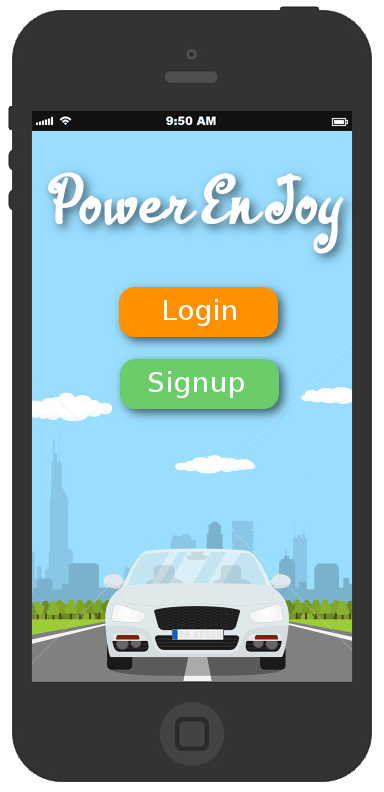
\includegraphics[width=0.2\textwidth]{mockup/1Login.png}
	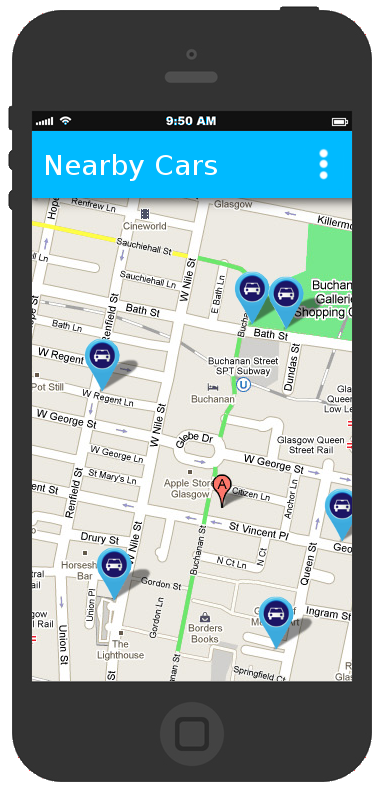
\includegraphics[width=0.2\textwidth]{mockup/2MainClient.png}
	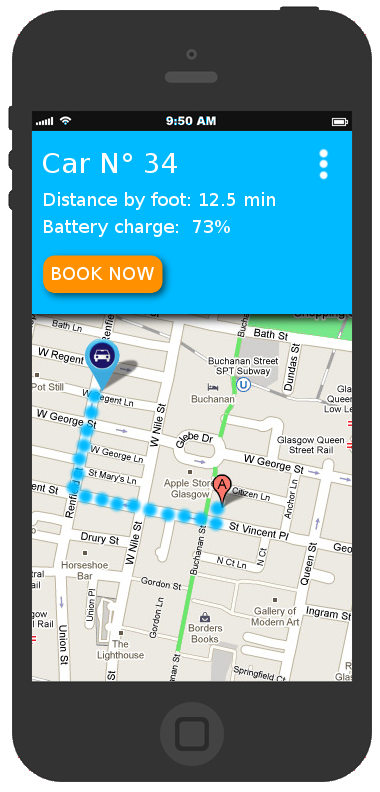
\includegraphics[width=0.2\textwidth]{mockup/3CarSelected.png}
	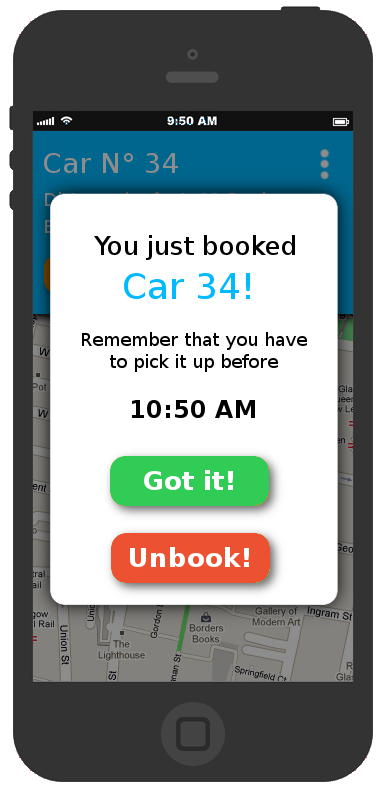
\includegraphics[width=0.2\textwidth]{mockup/4CarBooked.png}
	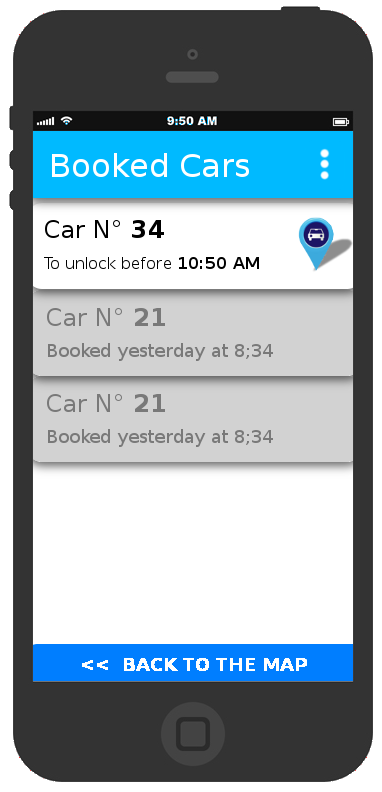
\includegraphics[width=0.2\textwidth]{mockup/5CarBookedList.png}
	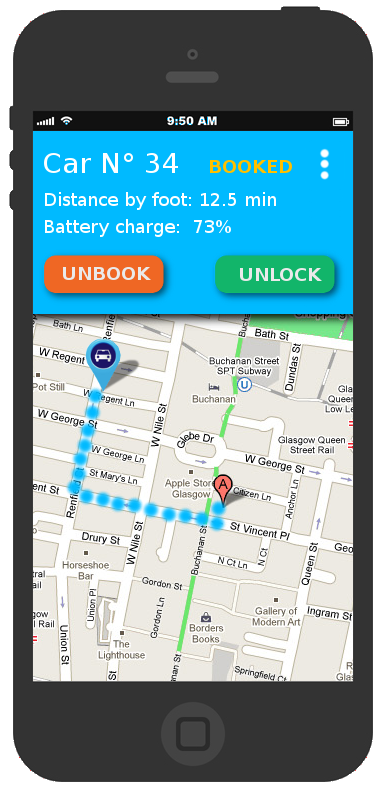
\includegraphics[width=0.2\textwidth]{mockup/6CarBookedSelected.png}
	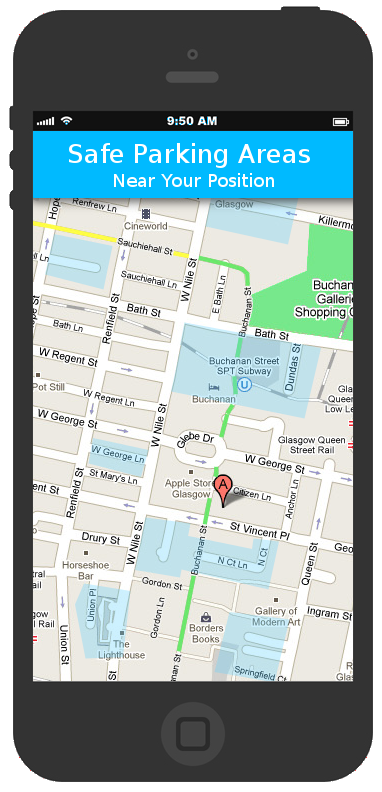
\includegraphics[width=0.2\textwidth]{mockup/7WhileDriving.png}
	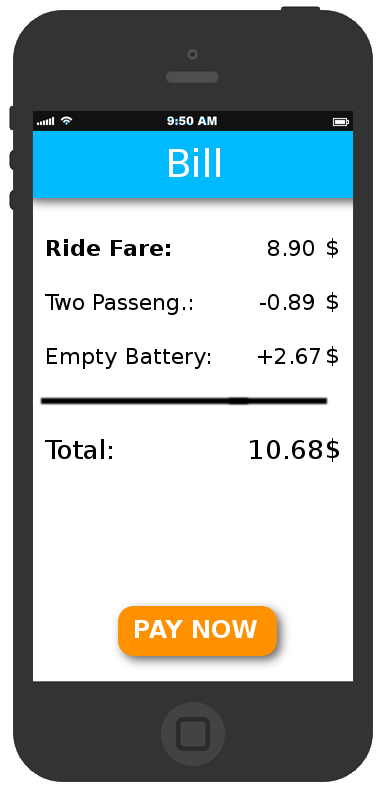
\includegraphics[width=0.2\textwidth]{mockup/8Bill.png}
	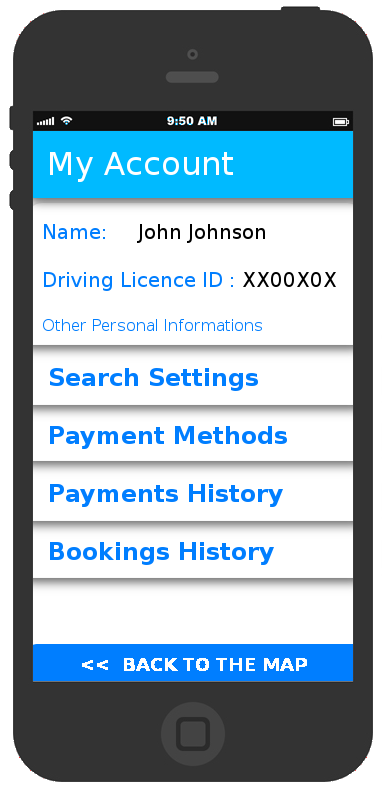
\includegraphics[width=0.2\textwidth]{mockup/9MyAccount.png}
	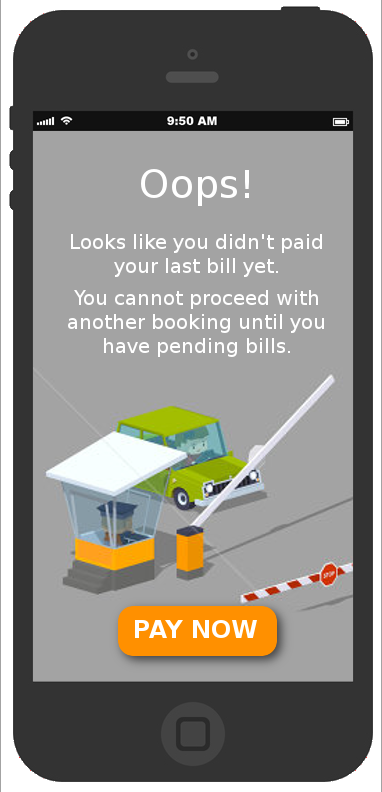
\includegraphics[width=0.2\textwidth]{mockup/10PendingBills.png}
	
\end{figure}
\subsubsection{Staff's App Interface}
%\end{comment}
  

\newpage
\section{Scenarios, Use Cases and UML Diagrams}

\subsection{Scenarios}

\subsubsection{Scenario 1}
John needs to go from the airport, which locates inside the city's boundaries, to his home. He is already a user of \pecomma so he opens the app and looks for some available cars in its area. He opens the map and finds there are 8 available cars in a 10-minutes walk distance from his home: 6 almost fully charged and 2 with about half charge left. He chooses the nearest full charged car and reserves it; then takes his luggage and reach the car within 15 min, leaving its phone's GPS active. Once near the car, the car is automatically unlocked: John can leave his luggage in the luggage van, enter the car and drive to the airport.

Once there, John parks correctly the car in a safe area, as indicated by the car's onboard system. John exits the car, takes his luggage out and uses the app to lock the car, which has still 60\% of battery charge left. Once the lock is confirmed he receives the bill, calculated on the lenght and duration of the ride, and a 20\% discount as a bonus to have left the car with more than 50\% of battery charge.

John pays the bill immediately through the app.

\subsubsection{Scenario 2}
John want to go from his home to the airport, which locates inside the city's boundaries, to bring two friends home. He reserves the nearest car and within 10 minutes he started his ride to the airport.

Once there, the car's onboard system tells him that there is a charging station nearby the airport. So John drives to the parking area nearby the charging station, parks, exits and plugs the car to the power grid. Then he locks the car.
Once the lock is confirmed, he receives the bill, calculated on the distance and the time of the ride, and receives a 30\% discount as bonus for plugging the car to the grid.

While waiting for his friends, he reserves another car for coming back, but the plane is late and the reservation, which lasts one hour, expires. John receives a little penalty for the expired reservation and pays it immediately; then reserves another car.

When his friends arrive, they all reach the car within 30 minutes from the second booking: they all enter and drive to his friends' home. When exiting, the car has about 40\% of charge left, but there are no charging stations nearby, so John parks it in a safe area, exit, take luggages out and locks the car. The app sends him the bill and applies a 10\% discount as a bonus for bringing at least two friends on the same ride.


\subsubsection{Scenario 3}
Bob has an exam at 8 a.m., but the morning train is very late. So he decides to user \pe to go to the university by car. He look for cars nearby, but he finds there is only one car left with about 40\% of residual charge. He reserves it anyways and within 5 minutes he started his drive to the university.

He is in a hurry, so drives very badly and commits some infractions, that gets recorded by the police. The policeman who is taking care of Bob's infractions looks in the police's databases for the owner of the car he spotted and sends the fine to \pe offices.

Once near his destination, the car's onboard system tells him that there is a charging station at about 10 minutes by foot from the university, and a parking area right in front of the entrance of the university. At the end of the ride, the car has only 15\% of residual charge.

Bob doesn't care and parks the car in front of the university, then exits and locks the car. The app confirms the lock and send him the bill, 30\% overpriced for having left the discharged car not plugged to the power grid, but at least he is in time for the exam.

At the end of the day, the fine has been processed by both the police officers and \pecomma so Bob receives a notification with the fine he received, some details about it, and the choice to pay it immediately or to go to the nearest police office to make an inquiry about it.


\subsubsection{Scenario 4}
it is a sunny Sunday and Charlie wants to go with his family in the countryside. He has no car, but he doesn't want to go there by train: so he decides to use \pe to do his trip. He finds a fully charged car near his house, reserves it and within 20 minutes he started his drive, heading outside the city's boundaries.

Once he crossed the boundaries, the car's onboard system informs him that he is not allowed to go that far and, if he will not go back into the boundaries within 10 minutes, he is going to be fined and, if stays far from the city for more than 24 hours, eventually prosecuted by law for having stolen the car. He does not care and continues his trip. After 10 minutes, he receives a notice that he is gonna be fined for the time he is spending outside the city.

At the end of the day, Charlie goes back home with his family. He parks the car in a safe area near his house, exits with all his family and locks the car: now he receives the bill, that is the basic price of the ride plus:
\begin{itemize}
	\item a 10\% discount for having brought many people on the car
	\item a 30\% overprice for having left the car discharged far from a charging station
	\item a heavy fine for having brought the car out from the city boundaries.
\end{itemize}
Charlie tries to pay, but his payment fails because the rechargeable credit card he connected to the app is empty. So he gets a notice from \pe that he is temporary banned from the service until he manages to pay the last pending bill.

\subsubsection{Scenario 5}
Harry is a staff operator of \pecomma in charge of re-chargin cars in-place when required. He has just completed another task in Charlie's neighborhood, so he opens the app and looks for any other pending issues to solve.

The app gives him a list of issues near him: two discharged cars left far from a power station, one parked near a power station that needs to be plugged, a Technical Issue and a car parked outside from a safe area. Harry filters the issues based on their Exception status, in order to see only issues related to recharging, and gets a list of the three discharged cars. He takes in charge Charlie's discharged car, which is the nearest, pressing the button on his app's interface. The app shows him the way and Harry goes for that car.

Once near the car, Harry plugs the car to his portable battery and charges it until it's almost full. Then changes manually the status of the car from Not Available to Available: but the system does not confirm the operation, because it cannot detect the residual charge of the battery. The Exception status of the car gets set to Mechanical Issue, but Harry has no means to fix that problem: so he does not take charge of the new issue and goes for another car to charge.


\subsubsection{Other scenarios}


Possible scenarios (REMOVE THIS LIST ONCE DONE)
\begin{enumerate}
	\item User rents a car in time, reach it in time, unlock, starts, ride, park in a safe area, exit, pay (1)
	\item User rents a car in time, reach it in time, unlock, starts, ride, park in a safe area, exit, PLUG IT, pay less. (2)
	\item User WITH FRIENDS rents a car in time, reach it in time, unlock, starts, ride, park, exit, pay less. (2)
	\item User rents a car in time, DON'T REACH IT IN TIME, pays penalty. (2)
	\item User rents a car in time, reach it in time, unlock, starts, ride, park in a safe area, exit, DON'T PLUG even if empty, pay more. --> \textbf{Not wrote}
	\item User rents a car in time, reach it in time, unlock, starts, ride, park in a safe area FAR FROM PLUG WHEN EMPTY, exit, pay more. (3)
	\item User tries to rent a car in time but NO CARS ARE AVAILABLE nearby. \textbf{Not wrote}
	\item User rents a car in time, reach it in time, unlock, starts, ride OUTSIDE THE CITY (4)
	\item User rents a car in time, reach it in time, unlock, starts, ride, park in an UNSAFE AREA, exit, pay. \textbf{Not wrote}
	\item User commits infraction while driving a \pe car. (3)
	\item User rents a car in time, reach it in time, unlock, starts, ride, park in a safe area, exit, but FAILS TO PAY. (4)
\end{enumerate}



\subsection{Use Case Diagram}


\subsection{Other UML Diagrams}
\subsubsection{Class Diagram}
\subsubsection{Sequence Diagram}
\subsubsection{Activity Diagram}
\subsubsection{State Diagram}



\newpage
\section{Alloy Model}

\newpage
\section{Hours}

\begin{itemize}
	\item SZ: 4h on 1/11
	\item SZ: 4h on 4/11
	\item SZ: 6h on 5/11
	\item SZ: 4h on 7/11

\end{document}
